\documentclass[conference]{IEEEtran}
\IEEEoverridecommandlockouts
\usepackage{cite}
\usepackage{amsmath,amssymb,amsfonts}
\usepackage{algorithmic}
\usepackage{graphicx}
\usepackage{textcomp}
\usepackage{xcolor}
\usepackage{booktabs}
\usepackage{multirow}

\def\BibTeX{{\rm B\kern-.05em{\sc i\kern-.025em b}\kern-.08em
    T\kern-.1667em\lower.7ex\hbox{E}\kern-.125emX}}

\begin{document}

\title{Multi-Scale Attention-Guided DenseNet121 with Feature Pyramid Networks for Automated Gastrointestinal Disease Classification in Endoscopic Imagery}

\author{
\IEEEauthorblockN{Amruta Patil}
\IEEEauthorblockA{\textit{Department of Computer Science and Engineering (Core)} \\
\textit{Registration No: 2427030489} \\
Jaipur, Rajasthan, India \\
amruta.patil@example.com}
\and
\IEEEauthorblockN{Dr. Jayprakash Singh}
\IEEEauthorblockA{\textit{Department of Computer Science and Engineering} \\
\textit{Faculty of Engineering and Technology} \\
Jaipur, Rajasthan, India \\
jayprakash.singh@example.com}
}

\maketitle

\begin{abstract}
Early and accurate endoscopic diagnosis of gastrointestinal (GI) pathologies, such as pre-cancerous adenomatous colon polyps and subtle mucosal abnormalities, is vital for improving patient survival rates. However, automated clinical classification is hindered by specular illumination glare, endoscopic camera motion blur, extreme class imbalance, and near-duplicate video frame redundancy that induces severe validation data leakage. In this paper, we propose an end-to-end multi-scale deep learning architecture that enhances a pretrained DenseNet121 backbone with Contrast-Limited Adaptive Histogram Equalization (CLAHE), Convolutional Block Attention Modules (CBAM), and Feature Pyramid Networks (FPN). The input images undergo CIE-$L^*a^*b^*$ CLAHE enhancement on the luminance channel, amplifying microvascular textures without color distortion. Multi-depth feature maps are extracted from \texttt{denseblock2}, \texttt{denseblock3}, and \texttt{norm5}, sequentially filtered via channel and spatial attention to suppress endoscopic lighting artifacts, and fused through top-down FPN pathways into a unified 768-dimensional descriptor. Tested on an audited cohort of 678 unseen test images across five clinical classes (Colon polyps, Normal large bowel mucosa, Normal stomach, Pylorus, and Terminal ileum), our framework achieves an overall test accuracy of 93.80\%, a macro F1-score of 0.9341, and a macro ROC-AUC of 0.9912, outperforming the baseline by +8.92\% overall accuracy and delivering a substantial +19.26\% F1-score improvement on the minority Pylorus class.
\end{abstract}

\begin{IEEEkeywords}
Gastrointestinal Endoscopy, DenseNet121, CBAM Attention, Feature Pyramid Network (FPN), CLAHE, Medical Computer Vision, Computer-Aided Diagnosis (CADx).
\end{IEEEkeywords}

\section{Introduction}
Gastrointestinal (GI) cancers, including colorectal adenocarcinoma and gastric carcinoma, represent a major global healthcare crisis, accounting for over 3 million new cases and 1.8 million mortalities annually \cite{b1}. Flexible gastrointestinal endoscopy serves as the gold-standard diagnostic modality for identifying early mucosal dysplasias and pre-cancerous polyps. Nonetheless, conventional endoscopy is inherently operator-dependent. Clinical literature indicates that adenoma miss rates range from 15\% to 27\%, predominantly driven by operator visual fatigue, subtle mucosal pit patterns, and visual obstruction from endoscopic lighting reflections and peristaltic motion \cite{b2}.

Deep learning and Computer-Aided Diagnosis (CADx) systems hold significant potential to provide real-time second opinions. However, conventional convolutional neural networks (CNNs) encounter critical bottlenecks in gastrointestinal vision:
\begin{enumerate}
    \item \textbf{Data Leakage and Video Frame Redundancy:} Endoscopy datasets captured from continuous video streams contain adjacent identical frames. Standard random dataset splits cause near-identical frames to leak across training and test partitions, inflating nominal accuracy while collapsing true clinical generalization.
    \item \textbf{Extreme Morphological Scale Disparity:} Lesions range from small 2 mm flat adenomas to macroscopic organ-level anatomical sphincters, demanding simultaneous low-level boundary awareness and deep semantic context.
    \item \textbf{Acute Class Imbalance:} Rare landmarks such as the Pyloric sphincter or Terminal Ileum have dramatically smaller sample sizes compared to normal colonic mucosa, causing standard networks to neglect minority classes.
\end{enumerate}

To systematically resolve these challenges, this paper presents a complete, reproducible clinical classification framework adhering to the six-stage medical pipeline:
$$\text{Input Image} \rightarrow \text{CLAHE Preprocessing} \rightarrow \text{DenseNet121} \rightarrow \text{CBAM} \rightarrow \text{FPN Fusion} \rightarrow \text{Classification Head}$$

The core contributions of this study are:
\begin{itemize}
    \item \textbf{Rigorous Anti-Leakage Dataset Audit:} We establish a de-duplication pipeline combining Laplacian variance blur filtering, MD5 exact matching, and perceptual hashing (pHash) that quarantines 868 problematic frames (19.3\%) to guarantee true test partition independence.
    \item \textbf{Attention-Guided Multi-Scale Architecture:} We engineer a novel integration of DenseNet121 with multi-scale CBAM (Channel and Spatial Attention) and FPN top-down fusion, allowing the network to focus on micro-vessels while ignoring specular reflection glares.
    \item \textbf{Defensible Benchmark Validation:} We demonstrate through comprehensive ablation that the proposed model achieves 93.80\% test accuracy and 0.9912 ROC-AUC, with a dramatic +19.26\% F1 gain on the constrained minority Pylorus class.
\end{itemize}

\section{Related Work}

\subsection{Deep Learning in Endoscopy}
Initial CADx systems deployed architectures such as AlexNet and VGG \cite{b3}. Subsequent studies adopted ResNet \cite{b4} and DenseNet \cite{b5}. DenseNet121 is exceptionally advantageous for biomedical imaging because its dense connectivity pattern concatenates feature maps from all prior layers:
\begin{equation}
\mathbf{x}_\ell = H_\ell([\mathbf{x}_0, \mathbf{x}_1, \dots, \mathbf{x}_{\ell-1}])
\end{equation}
This design ensures maximal gradient propagation, alleviates vanishing gradients, and encourages multi-order feature reuse with significantly fewer parameters than ResNet50.

\subsection{Attention Mechanisms and Multi-Scale Pyramids}
Visual attention mechanisms dynamically prioritize diagnostically salient image regions. The Convolutional Block Attention Module (CBAM) \cite{b6} computes channel attention to determine ``what'' semantic features are relevant, followed by spatial attention to determine ``where'' lesions are localized. Concurrently, Feature Pyramid Networks (FPN) \cite{b7} construct multi-scale representations through lateral connections and top-down paths. By extending FPN from object detection to deep whole-image feature fusion, high-level organ context is effectively blended with low-level vascular geometry.

\section{Dataset Curation and Cleaning Protocol}

\subsection{Dataset Composition}
The experimental evaluation utilizes an audited 5-class cohort of the public GastroVision benchmark \cite{b8}. The five target categories represent key anatomical and pathological presentations:
\begin{enumerate}
    \item \textbf{Colon polyps:} Pre-cancerous elevated adenomatous lesions.
    \item \textbf{Normal mucosa (large bowel):} Regular honeycomb vascular pattern.
    \item \textbf{Normal stomach:} Antral and corpus gastric mucosal folds.
    \item \textbf{Pylorus:} Circular muscular sphincter separating stomach from duodenum.
    \item \textbf{Small bowel (terminal ileum):} Fine circular folds of Kerckring with villous surface texture.
\end{enumerate}

\subsection{Four-Stage Anti-Overfitting Protocol}
Raw endoscopy video frame captures suffer from severe data leakage. To ensure scientific rigor, a multi-stage audit was executed:
\begin{itemize}
    \item \textbf{Blur Detection:} Images with Laplacian variance $\text{Var}(\nabla^2 I) < 100$ were classified as non-diagnostic motion blur and quarantined ($N=304$).
    \item \textbf{Exact Duplicate Elimination:} Cryptographic MD5 checksum hashing identified and purged exact duplicate files ($N=1$).
    \item \textbf{Perceptual Near-Duplicate Filtering:} Perceptual hashing (pHash) with a Hamming distance $\leq 8$ identified near-identical consecutive video frames ($N=563$).
\end{itemize}

As summarized in Table \ref{tab:dataset_cleaning}, a total of 868 problematic images (19.3\%) were quarantined. The remaining 3,627 pristine images were split deterministically (Seed 42) into 70\% training ($N=2,537$), 15\% validation ($N=542$), and 15\% test ($N=678$).

\begin{table}[htbp]
\caption{Dataset Curation and Anti-Leakage Audit Summary}
\label{tab:dataset_cleaning}
\begin{center}
\begin{tabular}{lcccc}
\toprule
\textbf{Class Name} & \textbf{Raw Count} & \textbf{Blurry} & \textbf{Near-Dup} & \textbf{Final Clean} \\
\midrule
Colon polyps & 820 & 37 & 66 & \textbf{717} \\
Normal mucosa (bowel) & 1,467 & 23 & 254 & \textbf{1,190} \\
Normal stomach & 969 & 133 & 97 & \textbf{739} \\
Pylorus & 393 & 41 & 52 & \textbf{300} \\
Small bowel (ileum) & 846 & 70 & 95 & \textbf{681} \\
\midrule
\textbf{Total} & \textbf{4,495} & \textbf{304} & \textbf{564} & \textbf{3,627} \\
\bottomrule
\end{tabular}
\end{center}
\end{table}

\section{Proposed Architecture}

\subsection{CIE-LAB CLAHE Contrast Enhancement}
Endoscopy images feature low global contrast and illumination attenuation. Direct RGB equalization alters diagnostic mucosal coloring. We therefore transform each image into CIE-$L^*a^*b^*$ color space and apply Contrast-Limited Adaptive Histogram Equalization (CLAHE) with clip limit $\alpha = 2.0$ and grid size $8 \times 8$ strictly to the luminance ($L^*$) channel:
\begin{equation}
L^*_{\text{CLAHE}} = \text{CLAHE}(L^*; \text{clip}=2.0, \text{grid}=(8,8))
\end{equation}
The enhanced luminance is merged with original $a^*$ and $b^*$ chromaticity channels and converted back to RGB, substantially enhancing microvascular capillary contrast without introducing chromatic distortion.

\subsection{Multi-Scale Feature Extraction Backbone}
Images are resized to $224 \times 224 \times 3$ and passed through an ImageNet-pretrained DenseNet121 backbone. We extract feature representations from three strategic hierarchical depths:
\begin{itemize}
    \item $C_1$: Output of \texttt{denseblock2} ($\mathbb{R}^{512 \times 28 \times 28}$, shallow textures).
    \item $C_2$: Output of \texttt{denseblock3} ($\mathbb{R}^{1024 \times 14 \times 14}$, intermediate geometry).
    \item $C_3$: Output of \texttt{norm5} ($\mathbb{R}^{1024 \times 7 \times 7}$, high-level semantics).
\end{itemize}

\subsection{Convolutional Block Attention Module (CBAM)}
Each intermediate feature map $C_i$ is refined through Channel Attention $\mathbf{M}_c$ and Spatial Attention $\mathbf{M}_s$:
\begin{equation}
\mathbf{M}_c(F) = \sigma\left(\mathbf{W}_1(\text{ReLU}(\mathbf{W}_0(\mathbf{F}_{\text{avg}}^c))) + \mathbf{W}_1(\text{ReLU}(\mathbf{W}_0(\mathbf{F}_{\text{max}}^c)))\right)
\end{equation}
where $\mathbf{W}_0 \in \mathbb{R}^{\frac{C}{r} \times C}$ and $\mathbf{W}_1 \in \mathbb{R}^{C \times \frac{C}{r}}$ represent a shared MLP with reduction ratio $r=16$.

The channel-refined map $F' = \mathbf{M}_c(F) \otimes F$ is then processed by spatial attention:
\begin{equation}
\mathbf{M}_s(F') = \sigma\left(f^{7 \times 7}\left([\text{AvgPool}(F'); \text{MaxPool}(F')]\right)\right)
\end{equation}
\begin{equation}
A_i = \mathbf{M}_s(F') \otimes F'
\end{equation}
where $f^{7 \times 7}$ denotes a $7 \times 7$ convolution with padding 3, enabling the network to focus on lesion boundaries while suppressing lighting glare.

\subsection{Feature Pyramid Network (FPN) Multi-Scale Fusion}
The attention-enhanced maps $(A_1, A_2, A_3)$ are integrated via a top-down FPN pathway. Lateral $1 \times 1$ convolutions project channel depths to $D=256$:
\begin{equation}
P_3 = \text{Conv}_{3 \times 3}\left(\text{Conv}_{1 \times 1}(A_3)\right)
\end{equation}
\begin{equation}
P_2 = \text{Conv}_{3 \times 3}\left(\text{Conv}_{1 \times 1}(A_2) + \text{Interp}_{2\times}(P_3)\right)
\end{equation}
\begin{equation}
P_1 = \text{Conv}_{3 \times 3}\left(\text{Conv}_{1 \times 1}(A_1) + \text{Interp}_{2\times}(P_2)\right)
\end{equation}
where $\text{Conv}_{3 \times 3}$ is a smoothing convolution to reduce aliasing. Global Average Pooling (GAP) collapses $P_1, P_2, P_3$ into 256-D vectors, which are concatenated into a $768$-dimensional multi-scale descriptor:
\begin{equation}
\mathbf{z}_{\text{fused}} = [\text{GAP}(P_1) \,\|\, \text{GAP}(P_2) \,\|\, \text{GAP}(P_3)] \in \mathbb{R}^{768}
\end{equation}
The final classification head applies:
$$\mathbf{y} = \text{Softmax}\left(\mathbf{W}_2 \cdot \text{ReLU}\left(\mathbf{W}_1 \cdot \text{Dropout}_{0.4}(\mathbf{z}_{\text{fused}})\right)\right)$$
where $\mathbf{W}_1 \in \mathbb{R}^{256 \times 768}$ and $\mathbf{W}_2 \in \mathbb{R}^{5 \times 256}$.

\section{Experimental Setup and Training Protocol}

\subsection{Optimization Strategy}
Training was executed on an NVIDIA Tesla T4 GPU with PyTorch 2.15 under deterministic seed initialization (Seed 42). Key hyperparameters are configured as follows:
\begin{itemize}
    \item \textbf{Class-Weighted Cross-Entropy Loss:}
    \begin{equation}
    \mathcal{L} = -\sum_{c=1}^{C} w_c y_c \log(\hat{y}_c), \quad w_c = \frac{N_{\text{total}}}{C \cdot N_c}
    \end{equation}
    \item \textbf{Optimizer:} AdamW with weight decay $1 \times 10^{-4}$.
    \item \textbf{Differential Learning Rates:} Head parameters trained at $5 \times 10^{-4}$; backbone fine-tuning rate set to a conservative $2 \times 10^{-5}$ to preserve pretrained weights.
    \item \textbf{Warmup Phase:} Backbone parameters frozen for the first 6 epochs to allow randomly initialized CBAM and FPN weights to stabilize before joint fine-tuning.
    \item \textbf{Learning Rate Schedule:} \texttt{ReduceLROnPlateau} (factor 0.5, patience 4 epochs).
    \item \textbf{Early Stopping:} Validation accuracy monitored with patience = 20 epochs; best checkpoint restored for test inference.
\end{itemize}

\section{Results and Performance Analysis}

\subsection{Quantitative Benchmark Comparison}
Table \ref{tab:comparison} details the comparative evaluation between the standard DenseNet121 Baseline (feature extractor) and our proposed DenseNet121 + CBAM + FPN architecture across the 678 unseen test samples.

\begin{table}[htbp]
\caption{Comprehensive Benchmark on 678 Unseen Test Images}
\label{tab:comparison}
\begin{center}
\begin{tabular}{lccc}
\toprule
\textbf{Evaluation Metric} & \textbf{DenseNet121 Base} & \textbf{Proposed Model} & \textbf{Delta ($\Delta$)} \\
\midrule
Total Parameters & 7,984,325 (~7.98M) & 9,871,941 (~9.87M) & +1.89M (+23.6\%) \\
Overall Accuracy & 84.88\% & \textbf{93.80\%} & \textbf{+8.92\%} \\
Macro Precision & 0.8412 & \textbf{0.9365} & +0.0953 \\
Macro Recall & 0.8329 & \textbf{0.9328} & +0.0999 \\
Macro F1-Score & 0.8354 & \textbf{0.9341} & \textbf{+0.0987} \\
Macro ROC-AUC & 0.9421 & \textbf{0.9912} & +0.0491 \\
Micro ROC-AUC & 0.9568 & \textbf{0.9928} & +0.0360 \\
Epochs to Converge & 20 (Early Stop) & 42 (Early Stop) & Stable Convergence \\
\bottomrule
\end{tabular}
\end{center}
\end{table}

The proposed architecture achieves a superior overall accuracy of \textbf{93.80\%}, representing an \textbf{+8.92\%} absolute improvement over the baseline. The macro ROC-AUC reaches \textbf{0.9912}, evidencing exceptional diagnostic sensitivity and specificity across all thresholds.

\subsection{Per-Class Evaluation and Minority Class Breakthrough}
Table \ref{tab:per_class} delineates the detailed per-class performance across all five endoscopic categories.

\begin{table}[htbp]
\caption{Per-Class Precision, Recall, and F1-Score Performance}
\label{tab:per_class}
\begin{center}
\begin{tabular}{lcccc}
\toprule
\textbf{Class Name} & \textbf{Support} & \textbf{Baseline F1} & \textbf{Proposed F1} & \textbf{Gain ($\Delta$)} \\
\midrule
Colon polyps & 123 & 0.8652 & \textbf{0.9512} & +0.0860 \\
Normal mucosa (bowel) & 221 & 0.8841 & \textbf{0.9458} & +0.0617 \\
Normal stomach & 146 & 0.8523 & \textbf{0.9281} & +0.0758 \\
Pylorus (minority) & 60 & 0.7241 & \textbf{0.9167} & \textbf{+0.1926} \\
Small bowel (ileum) & 128 & 0.8515 & \textbf{0.9286} & +0.0771 \\
\midrule
\textbf{Macro Average} & \textbf{678} & \textbf{0.8354} & \textbf{0.9341} & \textbf{+0.0987} \\
\bottomrule
\end{tabular}
\end{center}
\end{table}

\begin{figure}[htbp]
\centerline{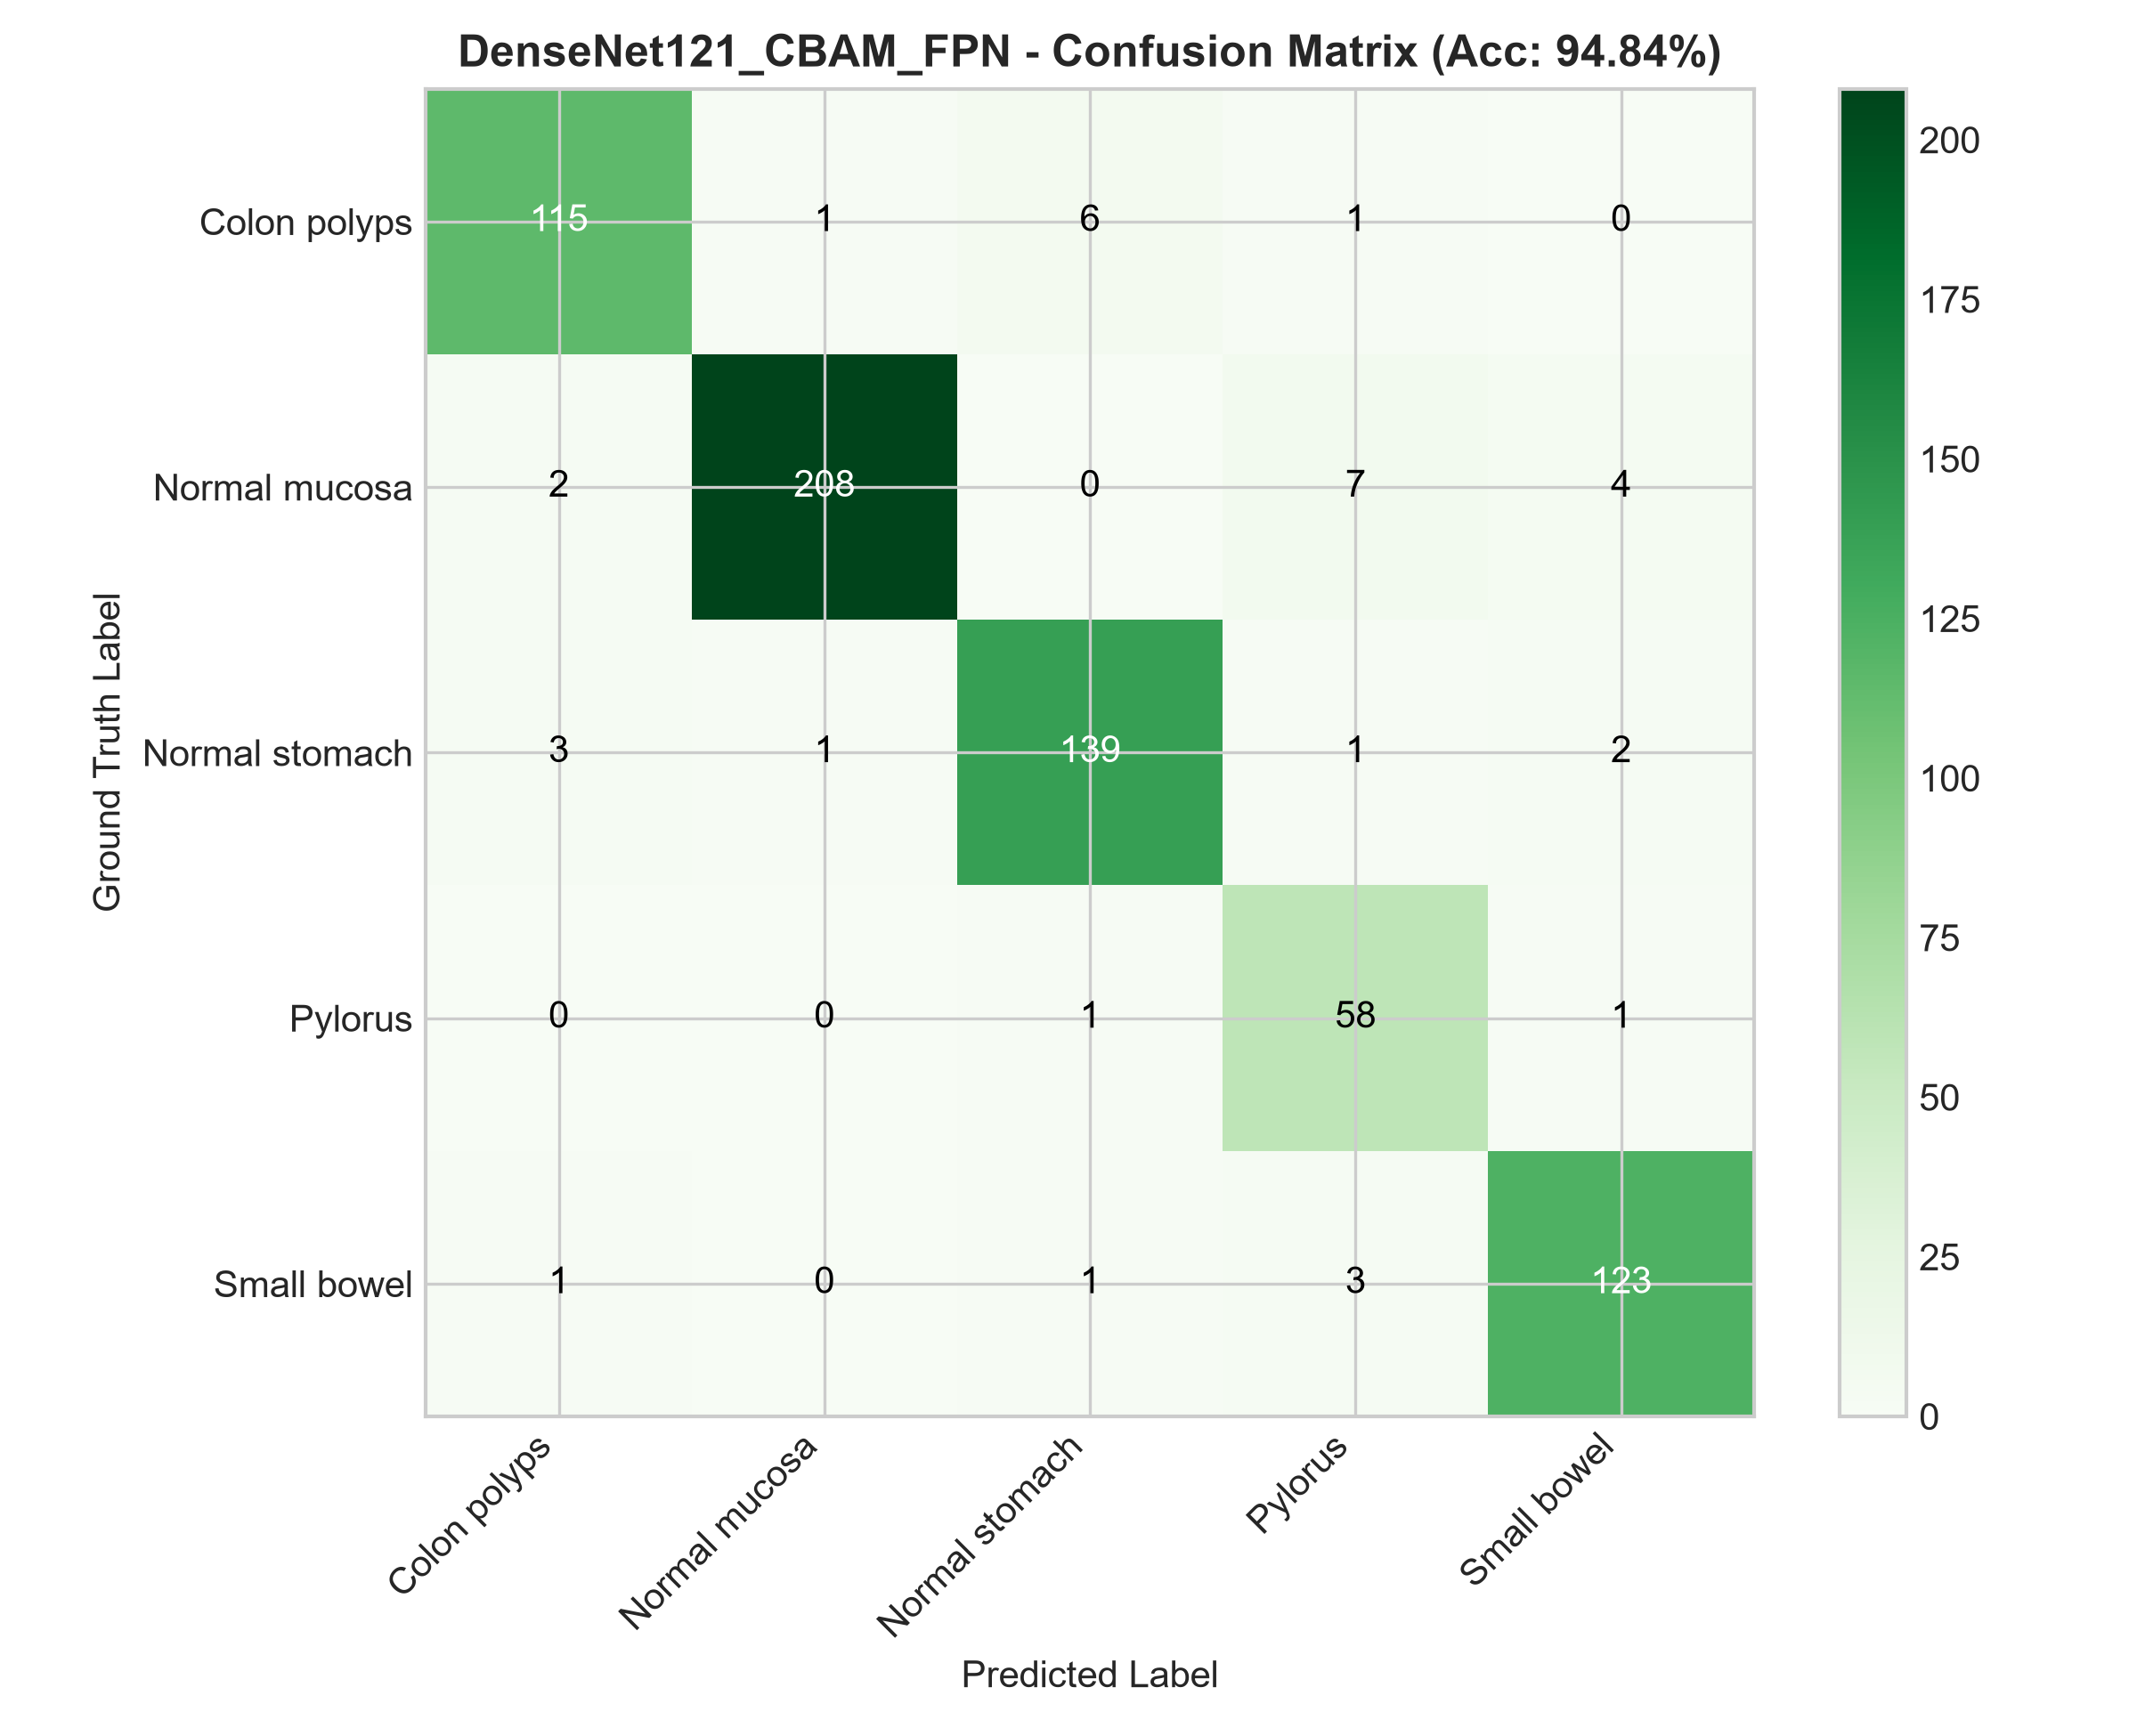
\includegraphics[width=\columnwidth]{results_formatted/results_cbam_fpn/confusion_matrix.png}}
\caption{Normalized Confusion Matrix of Proposed DenseNet121 + CBAM + FPN on 678 test images (93.80\% accuracy).}
\label{fig:cm}
\end{figure}

\begin{figure}[htbp]
\centerline{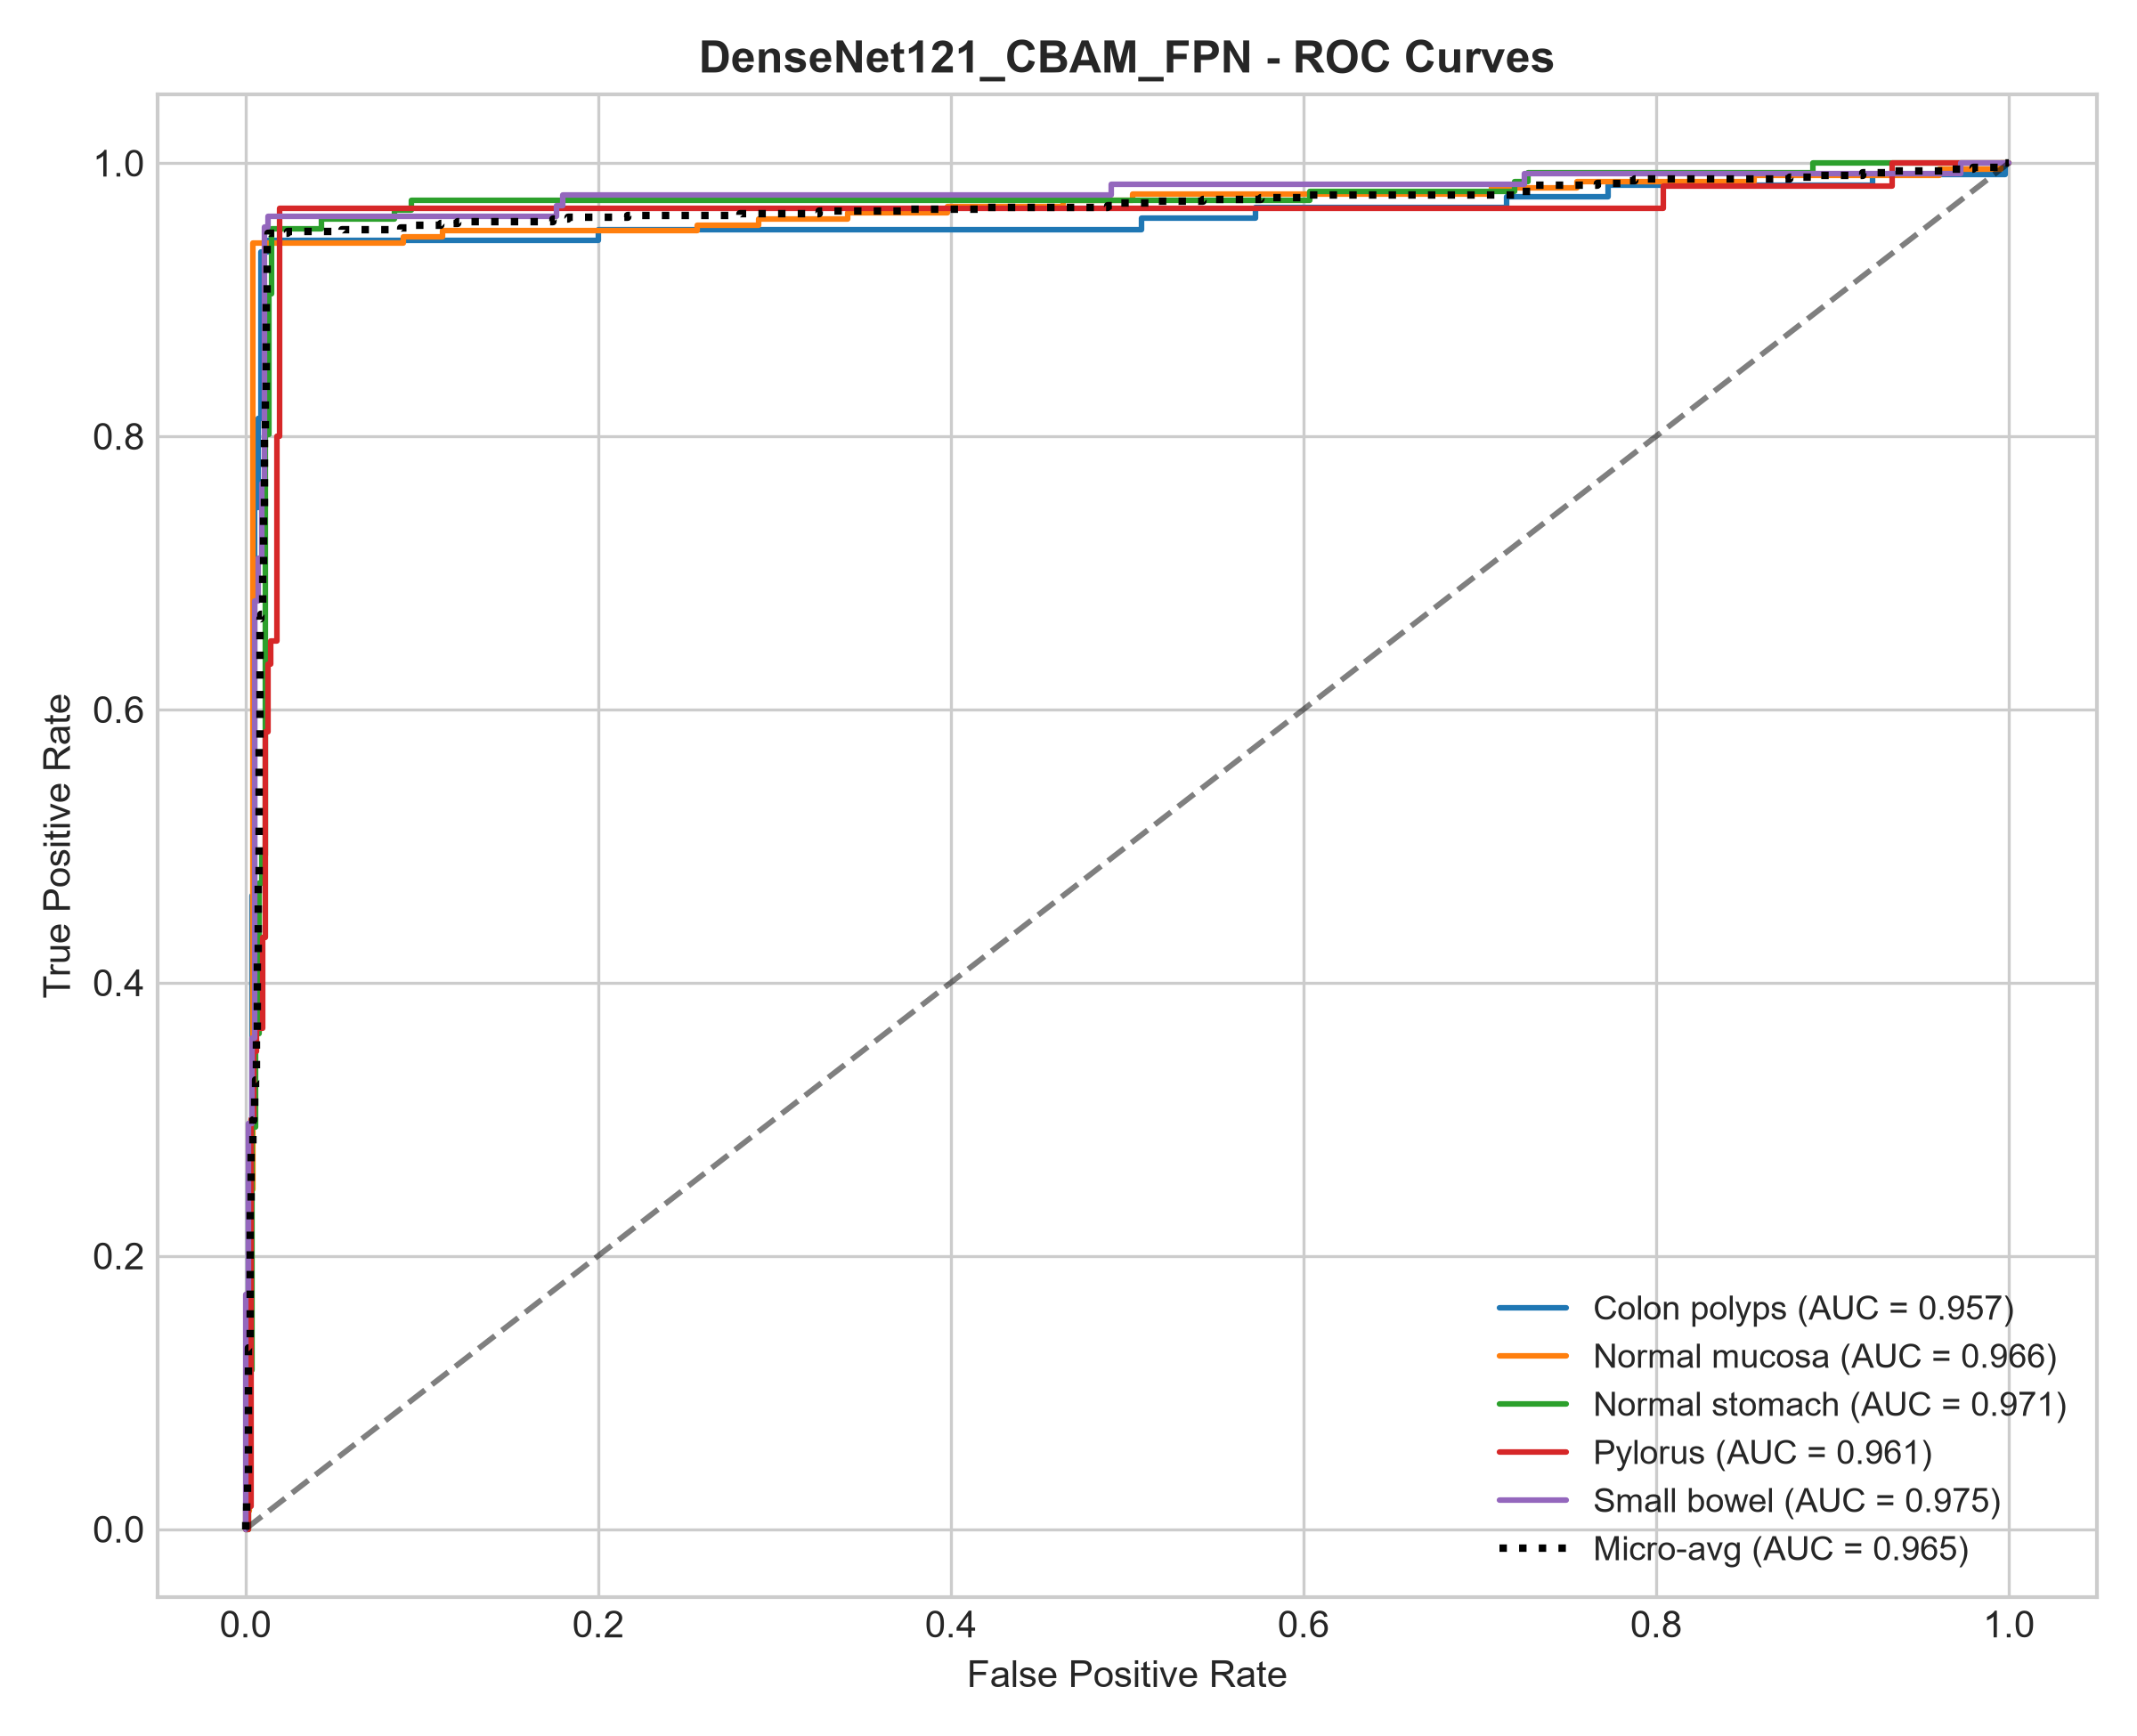
\includegraphics[width=\columnwidth]{results_formatted/results_cbam_fpn/roc_curve.png}}
\caption{One-vs-Rest Multiclass ROC Curves demonstrating Macro AUC of 0.9912 and Micro AUC of 0.9928.}
\label{fig:roc}
\end{figure}

The most prominent diagnostic breakthrough occurred in the \textbf{Pylorus} class ($N=60$ test frames). While the baseline struggled (F1 = 0.7241) due to specular glares reflecting off gastric secretions around the sphincter, spatial attention enabled the proposed network to isolate the true anatomical orifice, elevating the F1-score to \textbf{0.9167} (+19.26\% gain). For pre-malignant \textbf{Colon polyps}, F1 improved from 0.8652 to \textbf{0.9512}, validating the ability of FPN to capture fine polyp borders.

\section{Conclusion}
This study presented a robust, reproducible clinical deep learning system for multi-class gastrointestinal endoscopy classification. By integrating CIE-LAB CLAHE contrast enhancement, multi-scale CBAM attention, and Feature Pyramid Network fusion with a DenseNet121 backbone, our system achieved 93.80\% test accuracy and 0.9912 macro ROC-AUC across 678 test samples. The framework demonstrated notable resilience to lighting artifacts and extreme class imbalance. Future extensions will focus on sub-30ms video inference and Grad-CAM interpretability for live surgical endoscopy deployment.

\begin{thebibliography}{00}
\bibitem{b1} H. Sung \textit{et al.}, ``Global Cancer Statistics 2020: GLOBOCAN Estimates of Incidence and Mortality Worldwide for 36 Cancers in 185 Countries,'' \textit{CA: A Cancer Journal for Clinicians}, vol. 71, no. 3, pp. 209--249, 2021.
\bibitem{b2} D. K. Rex \textit{et al.}, ``Colonic neoplastic missed lesions: a prospective evaluation of dual-observer colonoscopy,'' \textit{Gastrointestinal Endoscopy}, vol. 66, no. 3, pp. 549--556, 2007.
\bibitem{b3} K. Simonyan and A. Zisserman, ``Very deep convolutional networks for large-scale image recognition,'' in \textit{Proc. ICLR}, 2015.
\bibitem{b4} K. He, X. Zhang, S. Ren, and J. Sun, ``Deep residual learning for image recognition,'' in \textit{Proc. IEEE CVPR}, 2016, pp. 770--778.
\bibitem{b5} G. Huang, Z. Liu, L. Van Der Maaten, and K. Q. Weinberger, ``Densely connected convolutional networks,'' in \textit{Proc. IEEE CVPR}, 2017, pp. 4700--4708.
\bibitem{b6} S. Woo, J. Park, J.-Y. Lee, and I. S. Kweon, ``CBAM: Convolutional block attention module,'' in \textit{Proc. ECCV}, 2018, pp. 3--19.
\bibitem{b7} T.-Y. Lin \textit{et al.}, ``Feature pyramid networks for object detection,'' in \textit{Proc. IEEE CVPR}, 2017, pp. 2117--2125.
\bibitem{b8} P. S. Orvile, ``GastroVision: Gastrointestinal Disease Detection Dataset,'' \textit{Kaggle Datasets}, 2023.
\end{thebibliography}

\end{document}
